\documentclass[10pt]{article}
\usepackage{/home/ford/Projects/transcripts/t2a/mea-pugna/NotesTeXV3/NotesTeX}

\graphicspath{ {/home/ford/Projects/transcripts/t2a/mea-pugna/img} }

\title{Título provisional}
\author{Marcos Ávila Navas}
\affiliation{I.E.S Los Colegiales}

\begin{document}

\maketitle

\flushbottom
\newpage
\pagestyle{fancynotes}

\part{Preambulo}

\section{Sobre este libro}

Este libro trata de recoger todos los temas que un estudiante de 2º de bachillerato puede encontrarse en las distintas asignaturas. Las asignaturas tratadas no son exhaustas: solo se recogen
\textbf{Matemáticas II}, \textbf{Física}, \textbf{Tecnología}, \textbf{Filosofía}, y \textbf{Lengua}. Es por tanto dirigido al itinerario tecnológico impartido en muchos centros, pero especialmente al impartido
en el I.E.S Los Colegiales.

\subsection{Cómo leer este libro}

Este libro intenta da una explicación profunda tal que el estudiante sea capaz de comprender la intuición que lleva al planteamiento de los problemas, el razonamiento tras los distintos resultados,
o las conclusiones del autor en cuestión. Cómo es así, mucho del contenido no es esencial y funciona para profundizar en el tema. Por lo tanto, lo único con valor de estudiar serán las secciones ``prácticas'' o ``resumen''.

Cabe también remarcar que el orden de los temas no es casualidad: de tanto en tanto se utilizarán conceptos ya trabajados en partes anteriores, tal que, por ejemplo, para mejor comprender por qué el
potencial gravitatorio tiende a 0 en el infinito, el lector será dirigido a la parte donde se trata tales cuestiones.

\newpage

\part{Matemáticas}

\section{Preludio}

Las areas de las matemáticas pertinentes a la selectividad son 4: \textbf{análisis real}, \textbf{geometría}, \textbf{algebra}, \textbf{probabilidad y estadísica}.

\subsection{Lógica proposicional de primer orden}

Se dice que las matemáticas son un lenguaje. Como tal, y aunque preferimos el lenguaje natural, y nos limitamos a este para todo lo relevante a la selectividad, es bueno familiarizarse con el lenguaje
matemático básico. Aunque existen varios ``lenguajes'' para las matemáticas, el más fácil, más usado, y el clásico es la ``\textbf{\textit{lógica proposicional de primer orden}}''.

En esencia, la lógica proposicional trata de construir ``\textit{proposiciones}'' utilizando un cierto conjunto de símbolos, los ``\textit{conectores lógicos}'' y los
``\textit{cuantificadores}''. Sin entrar en demasiado detalle, una proposición es una declaración con un valor de verdad (``\textit{Hoy hace sol}'', ``\textit{Sócrates es inmortal}'',
``\textit{Beethoven el perro fue un gran pianista}''\dots). Estas declaraciones naturalmente forman otras utilizando ``\textit{conectores lógicos}''. Por ejemplo, ``\textit{Mañana
lloverá y hoy hace sol}'' se puede descomponer en dos otras proposiciones, que si ambas son verdad harán la proposición total verdad. Cada conector lógico tiene asociado un símbolo
cómo ``$ \land $'' en el caso de ``y''.

Los conectores mas comunes son: conjunción (``\textit{\dots y \dots}'', ``$ \land $''), disyunción (``\textit{\dots o \dots}'', ``$ \lor $''), negación 
(``\textit{no \dots}'', ``$ \lnot $'') e implicación (``\textit{\dots por lo tanto \dots}'', ``$ \implies $'').

Por otra parte, también nos interesa hablar de para que cosas algo es verdad. Por ejemplo, ``\textit{\underline{Cualquier} número natural se puede factorizar en números primos}'' tiene un
sentido de extensión completamente distinto a ``\textit{\underline{Existen} 3 números enteros tal que la suma de los cuadrados de dos sean igual al cuadrado del tercero}''. Hay dos
tipos de cuantificadores: universal (``\textit{Cualquier ``x'', \dots}'', ``$ \forall x. \dots $'') y existencial (``\textit{Existe ``x'' tal que, \dots}'', ``$ \exists x. \dots $'').

Con esto, podemos adentrarnos un poco en la anatomía de la proposición. Una proposición tiene un ``sujeto'' (\textit{variables que representan de lo que se está hablando})
y un ``predicado'' (\textit{lo que se postula que las variables satisfacen}). Se dice que una variable es ``libre'' cuando aparece en el predicado sin haber sido cuantificada.
Típicamente nos interesan proposiciones sin variables libres, ya que es imposible deducir el valor de verdad de ``\textit{\underline{x} es mortal}'' si no sabemos de donde
procede \textit{x} (es decir, deberíamos añadir ``\textit{cualquier humano, llamese x, para el que \dots}'' o ``\textit{existe un humano, llamese x, para el que \dots}'').

El compendio anterior quizás no es suficiente para alguien no ya algo expuesto al lenguaje matemático. Para comprobar, uno debería de ser capaz de ``leer'' las siguientes ``oraciones''. \sn{La notación $ x \in X $ se introducirá en la sección posterior, significa ``x pertenece a X'' }

\begin{enumerate}

  \item \[ \forall x, y \in X.\; f(x) = f(y) \Rightarrow x = y \]

  \item \[ \forall y \in Y.\; \exists x \in X. \text{ tal que } f(x) = y \]

  \item \[ \exists \epsilon \in \mathscr{G}. \text{ tal que } \forall x \in \mathscr{G}.\; x \cdot \epsilon = \epsilon \cdot x = x \]

  \item \[ \forall \epsilon > 0.\; \exists \delta > 0. \text{ tal que } 0 < | x - a | < \delta \Rightarrow | f(x) - L | < \epsilon \]

\end{enumerate}

\subsection{Conjuntos}

En esencia, lo que las matemáticas clásicas \sn{Existen otras ``matemáticas'', por ejemplo la \href{https://ncatlab.org/nlab/show/constructive+mathematics}{constructiva}} son es el
estudio de ``conjuntos''. Un conjunto se puede pensar intuitivamente cómo un saco: una agrupación, desordenada, de elementos únicos (es decir, no permitimos elementos repetidos).
La notación básica de un conjunto es separar los elementos por comas y encapsular la enumeración con llaves, por ejemplo: $ \{2, 3, abc, \{\star\} \} $.

Sobre los conjuntos nos interesa fundamentalmente una cuestión: si algo pertenece a él o no. Esto se representa con un predicado el cuál se representa con la notación $ x \in X $
(se puede leer como ``x pertenece a X''). Por ejemplo, si $ X = \{2, 3, abc, \{\star\}\}  $ entonces $ 2 \in X $, pero no $ \star \in X $, lo correcto sería $ \{\star\} \in X $.

De aquí derivamos el concepto de función. Decimos que $ f : X \rightarrow Y $ es una función del conjunto $ X $ al conjunto $ Y $ a la asociación de cada elemento de $ X $ a un único
elemento de $ Y $. Por ejemplo, podemos considerar una función $ \chi : X \rightarrow Y $ de $ X = \{2, 3, abc, \{\star\}\} $ a $ Y = \{\text{true}, \text{false}\} $ que asocia a los
números de $ X $ a true y al resto de elementos a false. Otras veces consideramos funciones definidas por alguna fórmula. Si $ \mathbb{N} $ es el conjunto de números naturales,
$ \text{siguiente} : \mathbb{N} \rightarrow \mathbb{N} $ definida por $ \text{siguiente}(n) = n + 1 $ es una función.

Sobre las funciones es ineresante sacar 3 conjuntos:

\begin{itemize}
  \item El \textbf{dominio} ($\text{dom} f $): Si $ f : X \rightarrow Y $ es una función, $ \text{dom} f = X $ (es decir, el conjunto sobre el que $ f $ se define).
  \item El \textbf{codominio} ($\text{cod} f $): Si $ f : X \rightarrow Y $ es una función, $ \text{cod} f = Y $ (es decir, el conjunto al que $ f $ llega).
  \item La \textbf{imagen} ($\text{im} f $): Si $ f : X \rightarrow Y $ es una función, $ \text{im} f = f(X) $ (es decir, el conjunto en $ Y $ que $ f $ produce).
\end{itemize}

\newpage

\section{Análisis real}

El \textbf{análisis real} investiga los números reales, secuencias de estos, y funciones reales (funciones con dominio en $\mathbb{R}$).

\subsection{Funciones reales}

Una función real $ f $  es aquella tal que $ \text{dom} f =  X \subseteq \mathbb{R} $, es decir, cuyo dominio es $ \mathbb{R} $ o un subconjunto de este. 
Gracias a la estructura (\textit{topológica}) 
\sn{La topología es el estudio de espacios construidos por conjuntos. En topología $ \mathbb{R} $ se suele considerar como ``el espacio de la recta'', ``\textbf{la recta real}''}
de los números reales, podemos considerar la noción de \textbf{continuidad}:

\begin{definition}[Continuidad topológica]
  Decimos que una función real es continua en $ a $ si a cada intervalo abierto $ V $ que contiene a $ f(a) $ se le corresponde un intervalo abierto $ U $ que contiene a $ a $
  tal que $ f(U) \subseteq V $.
\end{definition}

Esta definición no es la estándar (la utilizada en selectividad será definida en la sección sobre límites). Sin embargo, nos da una buena intuición sobre lo que significa continuidad:
si pensamos en un intervalo abierto cómo una zona cercana a algún punto, una función continua, según esta definición, es aquella que zonas cercanas en el codominio se corresponden a
zonas cercanas en el dominio. Dicho de otra manera, si $ x $ está cercano a $ y $ en el dominio, $ f(x) $ esta cercano a $ f(y) $ en la imagen.

\subsubsection{En práctica}

En la selectividad no es raro un ejercicio que requiera calcular el dominio de una función. Para este fin, debemos identificar el dominio e imagen de todas las funciones con dominios restringidos involucradas y
restringir hasta que la imagen de la función que les sirve cómo argumento caiga en el dominio de estas funciones ``problemáticas''. A continuación una tabla con reglas de inferencia para los dominios:

\begin{center}
\begin{tabular}{| c | c |} 
 \hline
 $ f(x) $ & dom $ f $ \\
 \hline
 $ f_1(x) + f_2(x) $ & $ \text{dom} f_1 \cap \text{dom} f_2 $ \\
 $ f_1(x)f_2(x) $ & $ \text{dom} f_1 \cap \text{dom} f_2 $ \\
 $ f_1(x)/f_2(x) $ & $ (\text{dom} f_1 \cap \text{dom} f_2) \backslash \{f_2(x) = 0\} $ \\
 $ ax^b $ & $ \mathbb{R} $ \\
 $ \sqrt[2n]{x} $ & $ [0, +\infty) $ \\
 $ \sqrt[2n+1]{x} $ & $ \mathbb{R} $ \\
 $ a^x $ & $ \mathbb{R} $ \\
 $ \ln(x) $ & $ (0, +\infty) $ \\
 $ |x| $ & $ \mathbb{R} $ \\
 \hline
\end{tabular}
\end{center}

\subsection{Límites}

Los límites son la propiedad característica de los números reales \sn{Todo ``campo completo ordenado'' es isomórfico a $ \mathbb{R} $. }: el salto de los números racionales a los
números reales es precisamente requerir que toda secuencia (\href{https://ncatlab.org/nlab/show/Cauchy+sequence}{\textit{Cauchy}}) converja.

\begin{definition}[Secuencia]
  Una secuencia (de números reales) es una función de $ \mathbb{N} $ a $ \mathbb{R} $.

  Equivalentemente es una lista ordenada e infinita de números reales.
\end{definition}

\begin{definition}[Secuencia Cauchy]
  Se dice que una secuencia es \textit{Cauchy} cuando los números se acercan aribtrariamente. Si $ f : \mathbb{N} \rightarrow \mathbb{R} $ es una secuencia Cauchy:

  \[ \forall \epsilon \in \mathbb{R}. \exists N \in \mathbb{R}. \forall m, n \ge N. \; | f(m) - f(n) | < \epsilon  \]
\end{definition}

Con esta definición a mano, el límite de una función $ f $ cuando tiende a $ a $ es simplemente a lo que converja el aplicarle $ f $ a una secuencia Cauchy que converja a $ a $:

\begin{definition}[Límite de una función]
  Se dice que $ \lim_{x \to a} f(x) = L $ si:

  \[ \forall \epsilon > 0, \exists \delta > 0.\; | a - x | < \delta \Rightarrow | L - f(x) | < \epsilon \]
\end{definition}

En la práctica, hay veces que nos interesa investigar secuencias Cauchy que siempre sean mayores o menores que el número al que convergen:

\begin{definition}[Límites laterales de una función]
  Se dice que $ \lim_{x \to a^+} f(x) = L $ (convergencia por la derecha) si:

  \[ \forall \epsilon > 0, \exists \delta > 0. a < x < a +\delta \Rightarrow | L - f(x) | < \epsilon \]

  Dualmente, se dice que $ \lim_{x \to a^-} f(x) = L $ (convergencia por la izquierda) si:

  \[ \forall \epsilon > 0, \exists \delta > 0. a - \delta < x < a \Rightarrow | L - f(x) | < \epsilon \]
\end{definition}

También no son pocas las ocasiones donde nos interesa considerar el comportamiento de una función para números ``cada vez más grandes'':

\begin{definition}[Límites al infinito]
  Se dice que $ \lim_{x \to +\infty} f(x) = L $ si:

  \[ \forall \epsilon > 0. \exists N \in \mathbb{R}.\; x > N \Rightarrow | f(x) - L | < \epsilon \]

  Dualmente, se dice que $ \lim_{x \to -\infty} f(x) = L $ si:

  \[ \forall \epsilon > 0. \exists N \in \mathbb{R}.\; x < N \Rightarrow | f(x) - L | < \epsilon \]
\end{definition}

Todas estas definiciones serán unificadas para la resolución de problemas en lo que podemos llamar \textit{el algebra de los reales extendidos} ($ \bar{\mathbb{R}} $).

Finalmente, cabe replantear la definción de continuidad utilizando límties, ya que esta es la utilizada en la selectividad:

\begin{definition}[Continuidad]
  Decimos que una función real es continua en $ a $ si:

  \[ \lim_{x \to a^-} f(x) = f(a) = \lim_{x \to a^+} f(x) \]
\end{definition}

\subsubsection{Algebra de los reales extendidos}

Empezamos definiendo el conjunto sobre el cual definiremos las operaciones aptas para el cálculo de límites:

\begin{definition}[Los reales extendidos]
  Llamese $ \bar{\mathbb{R}} $ o ``reales extendidos'' al conjunto:
  \[ \bar{\mathbb{R}} = \mathbb{R} \cup \{+\infty, -\infty, \text{``Indet.''}, \text{``No existe.''}\}  \]
\end{definition}

Para describir el álgebra que nos interesa sobre el anterior conjunto, basta con definir cómo particípan los nuevos símbolos, y es que no modificamos las operaciones sobre
los números reales. Para este fin, basta con decir que los símbolos de infinito operan cómo uno esperaría ($ k + (\pm \infty) = \pm \infty $, $ k(\pm\infty) = \pm \infty $ \dots).
Los únicos casos donde la anterior intuición falla son en los casos ``indeterminados''.  % encontrar una lista de casos indeterminados para selectividad
Por último, el símbolo ``No existe'' viene a funcionar cómo un indicador de la divergencia de lo que se está intentando cálcular. Por ejemplo $ \cos{\pm\infty} = \text{``No existe''} $.

% Explicar el álgebra a fondo

\subsubsection{En la práctica}

Falta por explicar cómo pasar del cálculo de un límite a operar en el álgebra anteriormente descrito. Para lo cuál es suficiente decir que si se tiene $ \lim{x \to \alpha} f(x) $,
donde $ \alpha $ es o un real o un infinito, basta con sustituir $ \alpha $ por $ x $ en $ f(x) $ y operar siguiendo las reglas ya dichas. Si el resultado de operar es otra cosa
que no sea ``Indet.'', hemos terminado. En caso de un ``Indet.'', debemos trabajar $ f(x) $ hasta conseguir una expresión que al sustituir nos de el resultado deseado.

% Explicar transformaciones algebraicas típicas para arreglar f(x)

\subsection{Derivadas}



\subsection{Análisis de una función}

\subsection{Integrales}

\subsection{Ejercicios selectividad resueltos}

\begin{enumerate}
  \item \textbf{Madrid. Ordinaria 2025. Pregunta 2}: Un muro rectangular de la biblioteca pública del barrio se va a pintar con la ayuda de unos grafiteros. La dimensión del muro es de 3 metros de
        alto y 12 metros de largo. Colocando la esquina inferior izquierda del muro en el origen de coordenadas, se va a utilizar la curva
        \[ f(x) = \cos(\frac{\pi x}{9}) + 2 \]
        para diferenciar dos regiones del muro que serán pintadas con dos colores distintos. Se sabe que con un bote de spray se pueden pintar 3 metros cuadrados de superficie.
        \begin{enumerate}
          \item (0.75 puntos) Halle el valor máximo y el valor mínimo de la función $ f(x) $ en el intervalo $[0, 12]$. ¿Está la curva en este intervalo $ [0, 12] $ contenida completamente en el muro?
          \item (1.25 puntos) Halle el área que tienen que pintar de cada color.
          \item (0.5 puntos) Cuántos botes de spray se tienen que comprar como mínimo para pintar toda el área bajo la curva $ f(x) $?
        \end{enumerate}

        \begin{proof} % cambiar a ``solution''
          Por el teorema de Weierstrass, basta con estudiar los extremos del dominio y los máximos relativos para determinar los máximos y mínimos. Para este fin, nótese que $ f $ se define
          cómo una composición de funciones derivables, por lo que es derivable (asimismo continua). Por lo cuál, derivamos:
          \[ \frac{d}{dx} f = \frac{d}{dx} \cos(\frac{\pi x}{9}) + 2 = -\frac{\pi}{9} \sin(\frac{\pi x}{9}) \]
          A continuación, averiguamos los puntos críticos:
          \[ f'(x) = 0; \ -\frac{\pi}{9} \sin(\frac{\pi x}{9}) = 0; \ \frac{\pi x}{9} = n\pi; \ x = 9n \quad \text{donde } n \in \mathbb{Z} \]
          En concreto, en nuestro dominio encontramos dos puntos críticos, cuando $ n = 0 $ y $ n = 1 $.

          Desde este punto, basta con ordenar los valores de los puntos que nos interesan y tomar el mayor y el menor:
          \[ f(0) = 3 > f(12) = 1.5 > f(9) > 1 \]
          Por tanto, el valor máximo y mínimo de $ f $ es $ 3 $ y $ 1 $ cuando $ x = 0 $ y $ x = 9 $ respectivamente. Ya que $ 3, 1 \in [0, 3] $ y que $ f $ es continua,
          $ f $ es contenida completamente en el muro.
        \end{proof}

        \begin{proof}
          Para calcular el área de cada color, integramos y utilizamos la geometría rectangular del gráfico para derivar una área de otra:
          \[ A_1 = \int_0^{12} f(x) dx = \int_0^{12} \cos(\frac{\pi x}{9}) + 2 dx = \left[\frac{9}{\pi}\sin(\frac{\pi x}{9}) + 2x\right]_0^{12} \approx 21.51 m \]
          \[ A_T = A_1 + A_2; \ A_2 = A_T - A_1 = bh - A_1 \approx 14.48 m \]
        \end{proof}

        \begin{proof}
          Averiguamos la cantidad de botes utilizando que un bote puede pintar hasta 3 metros cuadrados de superficie:
          \[ n_{\text{botes}} = \lceil \frac{A_1}{\text{area}\backslash\text{bote}} \rceil = 8 \text{ botes}\]
        \end{proof}
\end{enumerate}


\section{Geometría}

\section{Algebra}

\section{Estadística y probabilidad}

\newpage

\part{Física}

\section{Preludio}

Las áreas de la física pertinentes a la selectividad son \dots : \textbf{Campo gravitatorio, campo eléctrico y campo magnético}, \dots.

\section{Campo}

\subsection{Mecánica clásica}

El campo gravitatorio es un campo vectorial en la mecánica clásica \sn{en la teoría de relatividad general es un \textbf{campo tensorial} }, y utilizamos los tres \textit{versores}
estándar: $ \hat{i}, \hat{j}, \hat{k} $.

Dentro del campo gravitatorio todas las fuerzas son atractivas y son resultantes de la masa de los objetos, que aproximamos cómo partículas puntuales.

\subsubsection{Momento lineal y angular}

\begin{definition}[Momento Lineal]
  El momento lineal $ \vec{p} $ es una magnitud vectorial que representa la inercia de un cuerpo, su resistencia a cambiar su estado de movimiento.
  
  $$ \vec{p} := m \vec{v} $$
\end{definition}

\begin{theorem}[Variacion del momento lineal]
  La variacion del momento lineal es precisamente la fuerza responsable del movimiento.
\end{theorem}

\begin{proof}
  $$ \frac{d \vec{p}}{dt} = \frac{d(m \vec{v})}{dt} = m \frac{d \vec{v}}{dt} = m \vec{a} = \vec{F} $$
\end{proof}

En un movimiento curvilíneo, $ \vec{p} $ cambia continuamente, lo cuál lo explicamos con una nueva magnitud:

\begin{definition}[Momento Angular]
  El momento angular $ \vec{L} $ caracteriza las propiedades de inercia de un cuerpo que gira respecto a un punto.
  
  $$ \vec{L} := \vec{r} \times \vec{p} $$
\end{definition}

En un movimiento circular podemos simplificar la definición de la magnitud del momento angular, ya que:

$$ L = r p \sin{\alpha} = r p \sin{90} = r p = r m v $$

\begin{definition}[Fuerza central]
  Fuerza central es aquella cuya direción es siempre a un punto fijo y cuya magnitud solo depende de la distancia a ese punto.
\end{definition}

\begin{theorem}[Conservación del momento angular]
  Para un cuerpo sometido a fuerzas centrales la variación del momento se anula.
\end{theorem}

\begin{proof}
  $$ \frac{d \vec{L}}{dt} = \vec{v} \times m \vec{v} + \vec{r} \times (m \vec{a}) = r \times \vec{F} $$

  Si ni $ \vec{r} = 0 $ ni $ \vec{F} = 0 $, entonces $ \vec{r} \times \vec{F} = 0 $  implica que $ \vec{r} $ y $ \vec{F} $ son paralelos (definición de fuerza central).
\end{proof}

\subsubsection{Energía y trabajo}

\begin{definition}[Trabajo]
  El trabajo se define de la siguiente forma:

  \[ W = \int_i^f \vec{F} \cdot d\vec{r} \]

\end{definition}

\begin{definition}[Energía y energía mecánica]
  Capacidad que tiene un cuerpo para realizar trabajo. La energía mecánica es aquella asociada al movimiento:

  \begin{itemize}
    \item \textbf{Energía cinética}: Energía que tiene un cuerpo en virtud a su velocidad: 
      \[ W = \int_i^f \vec{F} \cdot d\vec{r} = \int_i^f m\vec{a} \cdot d \vec{r} = \int_i^f m \frac{d\vec{v}}{dt} \cdot d \vec{r} = \int_i^f m \vec{v} \cdot d\vec{v} 
      = \frac{1}{2}m\left[v^2\right]_i^f = \Delta E_C \]
      \[ \implies E_C = \frac{1}{2} m v^2 \]
    \item \textbf{Energía potencial}: Energía que tiene un cuerpo en virtud a su posición en un campo conservativo:
      \[ W = -\Delta E_P \]
  \end{itemize}
  
  La suma de estas dos anteriores es la \textbf{energía mecánica}: 

  \[ E_M = E_C + E_P \]

\end{definition}

\subsection{Campo gravitatorio}

\subsubsection{Campo gravitatorio creado por masas puntuales}

\begin{definition}[Fuerza gravitacional]
  Fuerza resultante de las perturbaciones del campo gravitatorio.
  \[ \vec{F_g} = -G \frac{M m}{r^2} \hat{u_r} \]
\end{definition}

\begin{definition}[Intensidad del campo gravitatorio]
  Fuerza resultante por el campo gravitatorio por unidad de masa.
  \[ \vec{g} = \frac{\vec{F_g}}{m} = -G \frac{M}{r^2} \hat{u_r} \]
\end{definition}

\begin{remark}
  El principio de superposición aplica:
  \[ \vec{g_T} = \sum_i \vec{g_i} = -G \sum_i \frac{M_i}{r^2_i} \hat{u_{ri}} \]
\end{remark}

\subsubsection{Energía asociada al campo gravitatorio}

El campo gravitatorio es uno conservativo, por tanto:

\[ W = \int_i^f \vec{F_g} \cdot d\vec{r} = \int_i^f -G \frac{M m}{r^2} \hat{u_r} \cdot d\vec{r} = \int_i^f -G \frac{M m}{r^2} dr = -G M m \left[\frac{-1}{r}\right]_i^f = -\Delta E_P  \]

\[ \implies E_P = -G \frac{M m}{r} \]

\subsubsection{Potencial gravitatorio}

Considerar lo que hace una unidad de masa en el campo, así creando un ``espacio de gravedad'', nos lleva al concepto de potencial gravitatorio:

\begin{definition}[Potencial gravitatorio]
  Trabajo necesario para llevar una unidad de masa hasta el infinito a velocidad constante:

  \[ V = E_{P \infty} - E_P = G \frac{M}{r} \]
\end{definition}

Es fácil conectar la definción y la intuición considerando la expresión $ V m $.

\subsubsection{Campo gravitatorio de los cuerpos celestes}

El campo gravitatorio tal y cómo lo hemos presentado puede utilizarse para operar con cuerpos celestes (aproximadamente).

Para este fin, solemos igualar la fuerza centrípeta y la fuerza gravitatoria y desarrollar hasta tener una expresión en términos de los datos dados.

\begin{remark}
  La velocidad que obtenemos de esta manera es la órbital:
  \[ \vec{F_C} = \vec{F_G}; \ F_C = F_G; \ m \frac{v_o^2}{r} = G \frac{M m}{r^2}; \ v_o = \sqrt{G\frac{M}{r}}  \]
  El cálculo de la velocidad de escape, por ejemplo, se hace utilizando la ley de la conservación de la energía:
  \[ \Delta E_M \ge 0; \ \Delta E_C + \Delta E_P \ge 0; \frac{1}{2} m v_e^2 - G \frac{M m}{r} \ge 0; \ v_e \ge \sqrt{2 G \frac{M}{r}} \]
  Asimismo podemos proceder de la manera presentada para el cálculo de algún parametro para la transición entre órbitas.
\end{remark}

\subsubsection{Leyes de Kepler}

\begin{itemize}
  \item \textbf{Primera ley}: Todos los planetas se mueven alrededor del Sol siguiendo órbitas elípticas, y el Sol está en uno de los focos de la elipse.
  \item \textbf{Segunda ley}: Los cuerpos celestes se mueven con una velocidad areolar constante. Es decir, un mismo tiempo barre una misma área en cualquier punto de la órbita ($ \frac{dA}{dt} = cte. $)
  \item \textbf{Tercera ley}: Para todos los cuerpos celestes orbitando alrededor del mismo cuerpo, se cumple que:
    $$ \frac{T^2_1}{a^3_1} = cte. = \frac{T^2_2}{a^3_2} $$
\end{itemize}

El punto más alejado de una órbita elíptica es el afelio y el más cercano es el perihelio.

\subsection{Campo Eléctroestático}

El campo eléctrico es un campo vectorial al igual que el campo gravitatorio.

\subsubsection{Intensidad del campo electroestático}

\begin{definition}[Fuerza Eléctrica, Ley de Coulomb]
  La fuerza eléctrica es la resultante de las perturbaciones del campo electroestático.

  \[ \vec{F_e} = K\frac{Q q}{r^2} \cdot \hat{u_r} \]
\end{definition}

\begin{remark}
    Si se fija una dirección, es fácil ver que:
    \begin{itemize}
      \item \textbf{Si $ Q $ y $ q $ tienen mismo signo}: Entonces $ Q q > 0 $ por lo que  $ F_e > 0 $ (repulsión).
      \item \textbf{Si $ Q $ y $ q $ tienen distinto signo}: Entonces $ Q q < 0 $ por lo que  $ F_e < 0 $ (atracción).
    \end{itemize}

    Por lo que se justifica la regla ``similares se repelen y opuestos se atraen''.
\end{remark}

\begin{definition}[Intensidad eléctrica]
  Fuerza resultante por el campo eléctroestático por unidad de carga.

  \[ \vec{E} = \frac{\vec{F_e}}{q} = K\frac{Q}{r^2} \]
\end{definition}

\begin{remark}
  Nótese que si $ Q > 0 $  entonces $ \vec{E} $ y $ \hat{u_r} $ tendrán el mismo sentido mientras que si $ Q < 0 $ entonces $ \vec{E} $ y $ \hat{u_r} $ tendrán sentidos opuestos (demostración trivial).
\end{remark}

\begin{remark}
  También es importante remarcar que el principio de superposición aplica:
  
  \[ \vec{E_T} = \sum_{i} \vec{E_i} = K \sum_{i} \frac{Q_i}{r^2_i} \cdot \hat{u_{ri}}  \]
\end{remark}

\subsubsection{Energía asociada al campo eléctrico}

En la situación descrita, podemos llegar a una forma cerrada para el trabajo dentro del campo electroestático:

\[ W = \int_i^f \vec{F_e} \cdot d\vec{r} = \int_i^f K \frac{Q q}{r^2} \hat{u_r} \cdot d\vec{r} = \int_i^f K \frac{Q q}{r^2} dr = K Q q \left[ \frac{-1}{r} \right]_i^f  \]

\begin{definition}[Energía potencial eléctrica]
  La energía potencial eléctrica se define en virtud a que el campo electroestático es conservativo:

  \[ W_c = -\Delta E_P \qquad \text{ó} \qquad E_P = K \frac{Q q}{r} \]
\end{definition}

Intuitivamente, la energía potencial eléctrica es comparable a la gravitacional solo que cargas positivas ``suben el terreno'' mientras que cargas negativas lo bajan. De la misma manera que con los campos
gravitatorios, es fructífero considerar energía potencial por unidad de carga (A ser explicado a continuación).

\subsubsection{Potencial eléctrico}

\begin{definition}[Potencial eléctrico]
  Trabajo necesario para llevar una unidad de carga hasta el infinito a velocidad constante:

  \[ V = E_{P \infty} - E_P = K \frac{Q}{r} \]
\end{definition}

\begin{remark}
    Si se fija una dirección, es fácil ver que si $ Q $ y $ q $ tienen mismo signo ($ Q q > 0 $)
    \begin{itemize}
      \item \textbf{Si $ r_f > r_i $} (se aleja): Entonces $ W = -\Delta E_P = -q \Delta V > 0 $ (movimiento espontáneo).
      \item \textbf{Si $ r_f < r_i $} (se aleja): Entonces $ W = -\Delta E_P = -q \Delta V < 0 $ (se necesita suplir una fuerza).
    \end{itemize}
  Mientras que lo contrario es cierto si $ Q $ y $ q $ tienen distinto signo.
\end{remark}

\subsection{Campo magnético}

\newpage

\part{Tecnología}

\section{Preludio}

\section{Materiales y sus propiedades}

\subsection{Propiedades mecánicas de los materiales}

\begin{itemize}
  \item \textbf{Dureza}: Resistencia que ofrece un material a ser deformado o penetrado.
  \item \textbf{Elasticidad}: Propiedad general de los cuerpos sólidos, en virtud de la cual recobran más o menos de su extensión y forma, tan pronto como cesa la acción de la fuerza que las deformaba.
  \item \textbf{Plasticidad}: Propiedad general de lo que puede cambiar de forma y conservar esta de modo permanente si romperse.
  \begin{itemize}
    \item \textbf{Maleabilidad}: Propiedad de adquirir una deformación mediante una compresión sin romperse.
    \item \textbf{Ductilidad}: Propiedad de adquirir una deformación mediante tracción sin romperse.
  \end{itemize}
  \item \textbf{Resilencia}: Capacidad de absorver energía mecánica y recuperar su forma original despues de una deformación elástica.
  \begin{itemize}
    \item \textbf{A tracción}
    \item \textbf{A compresión}
    \item \textbf{A flexión}
    \item \textbf{A pandeo}
    \item \textbf{A torsión}
    \item \textbf{A la fatiga}
  \end{itemize}
\end{itemize}

\subsection{Ensayos de propiedades mecánicas}

\subsubsection{De tracción}

Conceptos previos:

\begin{itemize}
  \item \textbf{Tensión}: $ \sigma := \frac{F}{S} $
  \item \textbf{Alargamiento unitario}: $ \epsilon := \frac{\Delta l}{l_{0}} $
  \item \textbf{Estricción}: $ \epsilon_{t} := \frac{-\Delta S}{S_{0}} $
  \item \textbf{Modulo de Poisson}: $ \eta := \frac{\epsilon_{t}}{\epsilon} $
  \item \textbf{Módulo de elasticidad}: $ E := \frac{\sigma}{\epsilon} $
\end{itemize}

En el ensayo de tracción se somete a una probeta de forma y dimensiones normalizadas y del material a ensayar a un esfuerzo de tracción en la dirección de su eje,
de manera creciente y hasta romperla.

En un diagrama de tracción, se distinguen dos zonas características:

\begin{itemize}
  \item \textbf{Zona elástica (OE) [0, E]}
    \begin{itemize}
      \item \textbf{Zona de proporcionalidad (OP) [0, P]}: Es válido usar $ E $ como factor de conversión.
      \item \textbf{Zona no proporcional (PE) [P, E]}
    \end{itemize}
  \item \textbf{Zona plástica (ES) [E, S]}
    \begin{itemize}
      \item \textbf{Zona límite de rotura (ER) [E, R]}
      \item \textbf{Zona rotura efectiva (RS) [R, S]}
    \end{itemize}
\end{itemize}

Existen puntos entre E y S, cabe destacar:

\begin{itemize}
  \item \textbf{Rotura efectiva (R)}: Tras este punto, es inevitable la rotura.
  \item \textbf{Fluencia (F)}: (Solo para metales) Tras este punto, se produce un alargamiento sin que aumente la tensión aplicada.
\end{itemize}

El adjetivo ``límite'' a cualquiera de estos puntos refiere al valor de la tensión correspondiente al punto en la gráfica, se simboliza con $ \sigma _{(-)} $.

Otro nombre para $ \sigma_{E} $ es \textbf{tensión de admisión} ($ \sigma_{ad} $), y se puede aproximar al límite de proporcionalidad.

La \textbf{tensión de trabajo} es la tensión máxima a la que podemos someter una pieza respetando las recomendaciones y normas de seguridad, para calcularla, se aplica un coef. de seguridad $ N \in [1.2, 4] $.

\subsubsection{De dureza}

Brinell:

\begin{itemize}
  \item $ D := $ Diametro de bola.
  \item $ d := $ Diametro de la huella.
  \item  \textbf{Flecha}: $ f := \frac{1}{2} (D - \sqrt{D^2 - d^2}) $
  \item $ F := K D^2 $ donde $ K := $ cte. de ensayo.
  \item $ S := \pi D f $
  \item \textbf{Grado de dureza}: $ HB := \frac{F}{S} = \frac{F}{\pi D f} = \frac{2 F}{\pi D (D - \sqrt{D^2 - d^2})} $
\end{itemize}

La nomenclatura estandarizada tiene forma: ($HB$) HB($S | W$) ($D$) ($F$) ($t$), ($t$) solo es necesario si el tiempo no es entre 10 y 15 segundos, y donde $ S = $ Steel y $ W = $ Wolfram.

Vickers:

\begin{itemize}
  \item $ d := $ Diagonal de la huella.
  \item $ S := \frac{d^2}{2 \sin{68}} $
  \item \textbf{Grado de dureza}: $ HV := \frac{F}{S} = \frac{2 \sin{68º} F}{d^2} $
\end{itemize}

La nomenclatura estandarizada tiene forma: ($HV$) HV ($F$) ($t$), ($t$).

Rockwell:

\begin{itemize}
  \item $ HRC := 100 - 500h $
  \item $ HRB := 130 - 500h $
\end{itemize}

\subsection{De resilencia}

Consiste en medir la energía que absorbe un material al ser impactado. Se utiliza el péndulo Charpy.

Conceptos:

\begin{itemize}
  \item \textbf{Energía absorbida}: $ -\Delta E_p := - m g \Delta h $
  \item \textbf{Resilencia}: $ \rho := \frac{-\Delta E_p}{S}$, donde $ S := S_T - ent. $
\end{itemize}

\section{Máquinas térmicas}

\subsection{Principios fundamentales de termodinámica}

La termodinámica es la rama de la física que estudia las relaciones entre el calor, el trabajo, y la transferencia de energía.

\begin{definition}{Energía térmica ($ Q $)}{def1}
    En general,
    \[ Q := m C_E \Delta T \quad \text{donde } C_E := \text{calor específico} \]
    Para gases a volumen constante,
    \[ Q = m C_V \Delta T \quad \text{donde } C_V := \text{calor específico a volumen constante} \]
    Para gases a presión constante,
    \[ Q = m C_p \Delta T \quad \text{donde } C_p := \text{calor específico a presión constante} \]
\end{definition}

\begin{definition}{Energía interna ($ U $)}{def2}
    La energía interna ($ U $) es la que tiene una sustancia en virtud a su temperatura:
    \[ U := \sum E_c^{\text{partíc.}} \qquad\qquad \text{(Def. no utilizada en el temario)} \]
\end{definition}

A continuación, enumeramos los 3 principios básicos de la termodinámica:

\begin{enumerate}
    \item \textbf{Ley de la conservación de la energía}: La energía interna ($ U $) incrementa al añadir energía térmica al sistema, y hacer que el sistema realice trabajo la disminuye, ergo postulamos:
    \[ \Delta U = Q - W \]
    \item \textbf{Ley de la entropía}: La cantidad de entropía del universo tiende a incrementarse en el tiempo.
    \item \textbf{Principio del cero absoluto}: La entropía de un cristal perfecto de cualquier sustancia pura se aproxima a cero cuando la temperatura se aproxima al cero absoluto.
\end{enumerate}

Solo usaremos el primer principio para lo que prosigue.

\subsection{Transformaciones termodinámicas en los gases}

Asumimos la Ley de los gases ideales:

\begin{definition}{Ley de los gases ideales}{def3}
    Para un gas (ideal), se cumple:
    \[ pV = nRT \quad \text{donde } R = 0.082 \frac{L \cdot atm}{mol \cdot K} \]
\end{definition}

\subsubsection{Transformaciones isobáricas (presión constante)}

\[ pV = nRT; \; \frac{p}{nR} = \frac{V}{T} = cte. \; \Rightarrow \frac{V_1}{T_1} = \frac{V_2}{T_2} \]

Por la definición de presión ($ p := \frac{F}{S} $), tenemos:

\[ W := \int_{V_1}^{V_2} F \cdot dx = \int_{V_1}^{V_2} pS \cdot d x = \int_{V_1}^{V_2} p \cdot dV = p \Delta V \]

En cuanto a la gráfica $p$-$V$:

\begin{center}
 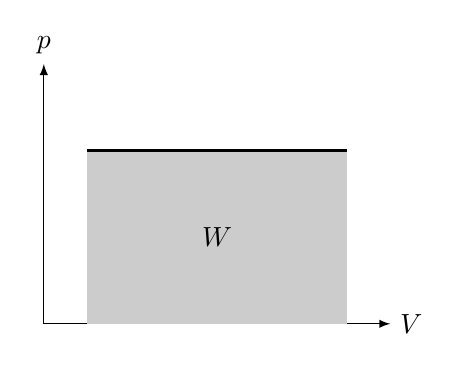
\begin{tikzpicture}[>=latex,scale=1.1]
   \draw[->] (0,0) -- (4,0) node[right] {$V$};
   \draw[->] (0,0) -- (0,3) node[above] {$p$};
 
   \fill[black!20] (0.5,0) rectangle (3.5,2);
 
   \draw[thick,black] (0.5,2) -- (3.5,2);
 
   \node at (2,1) {$W$};
 \end{tikzpicture}
\end{center}

\subsubsection{Transformaciones isotérmicas (temperatura constante)}

\[ pV = nRT = cte. \; \Rightarrow p_1V_1 = p_2V_2 \quad \text{ó} \quad \frac{p_1}{p_2} = \frac{V_2}{V_1} \]

Dado que, en estas condiciones, $ p = \frac{n R T}{V} $

\[ W := \int_{V_1}^{V_2} F \cdot dx = \int_{V_1}^{V_2} pS \cdot dx = \int_{V_1}^{V_2} p\cdot dV = \int_{V_1}^{V_2} \frac{n R T}{V} \cdot dV = n R T \ln \frac{V_2}{V_1} \]

En cuanto a la gráfica $p$-$V$:

\begin{center}
  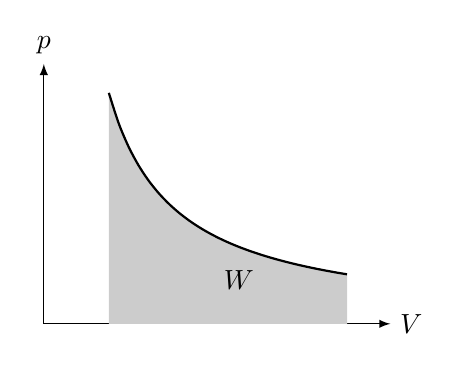
\begin{tikzpicture}[>=latex,scale=1.1]
    \draw[->] (0,0) -- (4,0) node[right] {$V$};
    \draw[->] (0,0) -- (0,3) node[above] {$p$};
    
    \fill[black!20,domain=0.75:3.5]
    (0.75,0)
    -- plot ({\x},{2/\x})
    -- (3.5,0)
    -- cycle;
    
    \draw[domain=0.75:3.5,smooth,variable=\x,thick,black]
    plot ({\x},{2/\x});
    
    \node at (2.25,0.5) {$W$};  
  \end{tikzpicture}
\end{center}

\subsubsection{Transformaciones isocóricas (volumen constante)}

\[ pV = nRT; \; \frac{V}{nR} = \frac{T}{p} = cte. \; \Rightarrow \frac{T_1}{p_1} = \frac{T_2}{p_2} \]

Es fácil ver que $ W = 0 $ ya que $ \Delta V = 0 $.

\[ Q = n C_V \Delta T \Rightarrow  (p_1 > p_2 \Leftrightarrow Q_1 > Q_2)\]

En cuanto a la gráfica $p$-$V$:

\begin{center}
\begin{tikzpicture}[>=latex,scale=1.1]
  \draw[->] (0,0) -- (4,0) node[right] {$V$};
  \draw[->] (0,0) -- (0,3) node[above] {$p$};

  \draw[thick,black] (2,0.5) -- (2,2.5);
  \node at (3,1.5) {$W=0$};
\end{tikzpicture}
\end{center}

\subsubsection{Transformaciones adiabáticas}

Sistemas perfectamente aislados o transformaciones instantáneas. Nada es constante.

\[ W = \frac{1}{1 - \gamma}(p_2V_2 - p_1V_1) \quad \text{donde } \gamma := \frac{C_p}{C_V} = \text{coef. adiabático} \]

Para el aire, $ \gamma \approx 1.4 $

En cuanto a la gráfica $p$-$V$:

\begin{center}
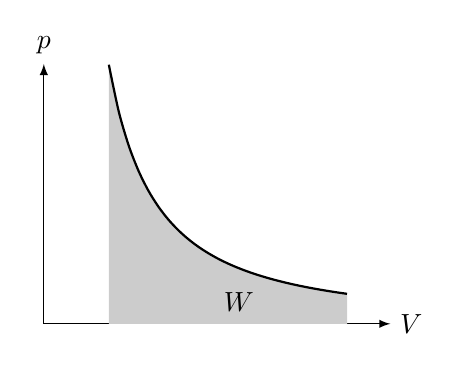
\begin{tikzpicture}[>=latex,scale=1.1]
  \draw[->] (0,0) -- (4,0) node[right] {$V$};
  \draw[->] (0,0) -- (0,3) node[above] {$p$};

  \fill[black!20,domain=0.75:3.5]
      (0.75,0)
      -- plot ({\x},{2/\x^1.4})
      -- (3.5,0)
      -- cycle;

  \draw[domain=0.75:3.5,smooth,variable=\x,thick,black]
      plot ({\x},{2/\x^1.4});

  \node at (2.25,0.25) {$W$};
\end{tikzpicture}
\end{center}

\subsection{Procesos reversibles e irreversibles}

Llamamos proceso reversible a aquel en el cuál en el proceso de transformación $ (p_0, V_0, T_0) \rightarrow (p, V, T) $ todos los estados intermedios son estables. Es decir, la transformación es lenta.

\subsubsection{Motores térmicos y máquinas frigoríficas}

Una máquina térmica basa su funcionamiento en el flujo de energía calorífica entre dos focos. Si saca calor de un foco caliente, lo vierte en otro frío, y aprovecha el trabajo resultante de la transformación, se llama \textbf{motor térmico}. Si por el otro lado saca calor de un foco frío utilizando trabajo y lo vierte en otro caliente, se llama \textbf{máquina frigorífica}.

En esta situación,

\[ W = Q_c - Q_f\]

\[ \eta := \frac{E_u}{E_a} = \frac{W}{Q_c} = 1 - \frac{Q_f}{Q_c} \]

\subsubsection{Ciclo ideal de Carnot}

Máximo rendimiento que se puede extraer de dos focos. El rendimiento es comúnmente aproximado tal que:

\[ \eta \approx 1 - \frac{T_f}{T_c} \]

Asumimos la transmisión calorífica perfecta en las expansiones y el aislamiento perfecto en las compresiones:

\begin{enumerate}
    \item \textbf{Expansión isotérmica}: Se aplica el calor del foco caliente, resultando en una expansión del gas a la misma temperatura que el foco caliente.
    \item \textbf{Expansión adiabática}: Se retira el foco caliente; el gas sigue expandiéndose debido a la energía cinética residual.
    \item \textbf{Compresión isotérmica}: Se aplica el calor del foco frío, retirando el calor del gas y dejándolo a la misma temperatura que la del foco frío.
    \item \textbf{Compresión adiabática}: Se retira el foco frío; el gas sigue comprimiéndose debido a la energía cinética residual.
\end{enumerate}

\begin{center}
\begin{tikzpicture}[>=latex,scale=1.1]
  \draw[->] (0,0) -- (4,0) node[right] {$V$};
  \draw[->] (0,0) -- (0,3) node[above] {$p$};

\end{tikzpicture}
\end{center}

\subsection{Motores de combustión interna}

Siempre nos vamos a encontrar con un pistón y una recámara. Por lo que distinguimos entre tipo de transformación que se produce en la aplicación del foco caliente, y número de movimientos del pistón (tiempos) en el que el ciclo se completa. 

\subsubsection{Motores de explosión}

Nos centramos en el ciclo de Otto.

\begin{itemize}
    \item \textbf{De 4 tiempos}: 
        \begin{center}
            \includegraphics[scale=0.5]{Ciclo_de_4_tiempos.JPG}
        \end{center}

        \begin{enumerate}
            \item \textbf{Fase de admisión}: transformación isobárica.
            \item \textbf{Fase de compresión}: transformación adiabática; transformación isocórica (explosión, combustión instantánea).
            \item \textbf{Fase de expansión}: transformación adiabática; transformación isopórica (apertura de la válvula).
            \item \textbf{Fase de escape}: transformación isobárica.
        \end{enumerate}
        
        \begin{center}
        \begin{tikzpicture}[>=latex,scale=1.1]
          \draw[->] (0,0) -- (4,0) node[right] {$V$};
          \draw[->] (0,0) -- (0,3) node[above] {$p$};
        
        \end{tikzpicture}
        \end{center}
   \item \textbf{De 2 tiempos}: 
        \begin{center}
            \includegraphics[scale=0.2]{Esquema-de-2-tiempos.jpg}
        \end{center}

        \begin{enumerate}
            \item \textbf{Fase de compresión y aspiración}: transformación adiabática; transformación isobárica.
            \item \textbf{Fase de explosión y escape}: transformación adiabática; transformación isobárica.
        \end{enumerate}
        
        \begin{center}
            \begin{tikzpicture}[>=latex,scale=1.1]
              \draw[->] (0,0) -- (4,0) node[right] {$V$};
              \draw[->] (0,0) -- (0,3) node[above] {$p$};
            \end{tikzpicture}
        \end{center}
\end{itemize}

\subsubsection{Motores de diesel}

Los motores diesel cambian la bujia que produce la explosión del combustible por un inyector (combustión progresiva).

\begin{itemize}
    \item \textbf{De 4 tiempos}:
        \begin{enumerate}
            \item \textbf{Fase de admisión}: transformación isobárica.
            \item \textbf{Fase de compresión}: transformación adiabática.
            \item \textbf{Fase de expansión}: transformación isobárica (combustión); transformación (adiabática).
            \item \textbf{Fase de escape}: transformación isocórica; transformación isobárica.
        \end{enumerate}
        \begin{center}
            \begin{tikzpicture}[>=latex,scale=1.1]
              \draw[->] (0,0) -- (4,0) node[right] {$V$};
              \draw[->] (0,0) -- (0,3) node[above] {$p$};
            \end{tikzpicture}
        \end{center}
    \item \textbf{De 2 tiempos}:
        \begin{enumerate}
            \item \textbf{Fase de compresión y aspiración}: transformación adiabática; transformación isocórica.
            \item \textbf{Fase de explosión y escape}: transformación adiabática; transformación isocórica.
        \end{enumerate}
        \begin{center}
            \begin{tikzpicture}[>=latex,scale=1.1]
              \draw[->] (0,0) -- (4,0) node[right] {$V$};
              \draw[->] (0,0) -- (0,3) node[above] {$p$};
            \end{tikzpicture}
        \end{center}
\end{itemize}

\subsubsection{Parámetros y magnitudes características}

\begin{itemize}
    \item \textbf{Calibre}: $ d := \text{diam.} $
    \item \textbf{PMS}: Punto muerto superior.
    \item \textbf{PMI}: Punto muerto inferior.
    \item \textbf{Carrera}: $ h := PMS - PMI$
    \item \textbf{Cilindrada}: $ V := \pi \frac{d^2}{4} h n \quad \text{donde } n := \text{núm. de cilindros} $
    \item \textbf{$V_c$}: Volumen cámara de compresión.
    \item \textbf{Relación de compresión}: $ RC := \frac{V_1 + V_c}{V_c} $
    \item \textbf{Gasto}: $ G := \frac{m_c}{t} $
    \item \textbf{Potencia absorbida}: $ P_a = G P_c \quad \text{donde } P_c = \text{poder calorífico} $
    \item \textbf{Momento de torsión}: $ M = F r $
    \item \textbf{Potencia útil}: $ P_u = M \omega $
\end{itemize}

\subsection{Motores de combustión externa}

Su utilidad es la generación eléctrica y de propulsor de aviones.

\subsubsection{Ciclo de Rankine (Turbina de vapor)}

\begin{center}
    \includegraphics[scale=0.3]{Ciclo_de_Rankine.jpg}
\end{center}

\begin{enumerate}
    \item \textbf{Caldera}: transformación isobárica: Absorción de calor en la caldera, comienza el cambio de fase, se produce vapor sobrecalentado.
    \item \textbf{Turbina}: transformación adiabática.
    \item \textbf{Condensación}: transformación isobárica; transformación isotérmica.
    \item \textbf{Bomba}: transformación isocórica.
\end{enumerate}

\begin{center}
    \begin{tikzpicture}[>=latex,scale=1.1]
      \draw[->] (0,0) -- (4,0) node[right] {$V$};
      \draw[->] (0,0) -- (0,3) node[above] {$p$};
    \end{tikzpicture}
\end{center}

\subsubsection{Ciclo de Brayton (Turbina de gas)}

\begin{center}
    \includegraphics[scale=0.5]{Ciclo_de_Brayton.png}
\end{center}

\begin{enumerate}
    \item \textbf{Compresor}: transformación adiabática.
    \item \textbf{Quemador}: transformación isobárica.
    \item \textbf{Turbina}: transformación adiabática.
\end{enumerate}

\begin{center}
    \begin{tikzpicture}[>=latex,scale=1.1]
      \draw[->] (0,0) -- (4,0) node[right] {$V$};
      \draw[->] (0,0) -- (0,3) node[above] {$p$};
    \end{tikzpicture}
\end{center}


\subsection{Bombas de calor}

La transmisión de calor de un foco frío a uno caliente no es espontánea. Por lo cual necesitamos realizar trabajo para que esto ocurra. Este trabajo será igual a la diferencia de calor de los
focos $ W = Q_C - Q_F $.

\subsubsection{Ciclo de refrigeración de Carnot}

Máxima eficiencia que se puede extraer de dos focos. El rendimiento es comúnmente aproximado tal que:

\[ \epsilon = \frac{E_u}{E_a} = \frac{Q_F}{W} = \frac{Q_C}{Q_C - Q_F} \approx \frac{T_C}{T_C - T_F} \]

Asumimos la transmisión calorífica perfecta en las expansiones y el aislamiento perfecto en las compresiones:

\begin{enumerate}
  \item \textbf{Compresión adiabática} Se realiza el trabajo comprimiendo el émbolo. Aumenta la temperatura y presión del gas.
  \item \textbf{Compresión isotérmica} Se aplica el foco caliente, que toma calor del gas.
  \item \textbf{Expansión isotérmica} Se retira el foco caliente, causando que el gas se expanda y disminuya su temperatura.
  \item \textbf{Compresión isotérmica} Se aplica el foco frío, que retira calor del gas.
\end{enumerate}

\begin{center}
    \begin{tikzpicture}[>=latex,scale=1.1]
      \draw[->] (0,0) -- (4,0) node[right] {$V$};
      \draw[->] (0,0) -- (0,3) node[above] {$p$};
    \end{tikzpicture}
\end{center}

\subsubsection{Ciclo de Rankine inverso}

\begin{enumerate}
  \item \textbf{Compresión adiabática}: El vapor saturado procedente del evaporador llega al compresor; aumenta su temperatura hasta alcanzar el punto
    correspondiente al vapor recalentado. Esta transformación se realiza con la aportación de trabajo externo ($ W $).
  \item \textbf{Transformación isobárica}: En el condensador, el vapor está a una temperatura mayor que la del ambiente, por tanto cede calor ($ Q_C $), manteniendo constante
    la presión, mientras se produce, primero, un enfriamiento seguido de una condensación hasta convertirse en líquido saturado. Al pasar de vapor a líquido hay una gran reducción
    de volumen, con lo cual el fluido pasa a un estado líquido a alta presión.
  \item \textbf{Expansión adiabática}: Se hace pasar el fluido por la válvula de expansión, donde se produce una transformación adiabática con un ligero aumento del volumen y
    gran disminución de presión y temperatura. Una parte del líquido se vaporiza, y en el punto 4 hay vapor húmedo.
  \item \textbf{Transformación isobárica} El vapor húmedo, a su paso por el evaporador, que se encuentra en el recinto que queremos refrigerar, absorbe calor del foco frío ($ Q_F $)
    por encontrarse a menor temperatura que éste. Se completa la vaporización del fluido a medida que aumenta su volumen hasta llegar a la entrada del compresor, donde comienza de
    nuevo el ciclo.
\end{enumerate}

Este ciclo puede servir tanto para refrescar en verano ($ Q_C = $ \textit{exterior}, $ Q_F =  $ \textit{interior}) como calentar en invierno ($ Q_C = $ \textit{interior},
$ Q_F =  $ \textit{exterior}). Asimismo tanto el evaporador como el condensador pueden intercambiar funciones. Concluimos que solo es necesario alternar el flujo del refrigerante
para alternar funciones.

\begin{center}
    \begin{tikzpicture}[>=latex,scale=1.1]
      \draw[->] (0,0) -- (4,0) node[right] {$V$};
      \draw[->] (0,0) -- (0,3) node[above] {$p$};
    \end{tikzpicture}
\end{center}

Cabe enumerar los distintos elementos presentes en la refrigeración por vapor. Estos son: compresor (puede ser centrífugo o volumétrico), condensador o evaporador (intercambiadores
de calor), válvula de expansión (mantiene la presión constante del refrigerante que se dirige hacia el evaporador).

\begin{center}
  \includegraphics[scale=0.5]{Ciclo_de_Rankine_inverso.png}
\end{center}

\newpage

\part{Historia de la Filosofía}

\section{Preludio}

Los autores filosóficos pertinentes a la selectividad son: \textbf{Platón, Descartes, Nietzsche y Ortega} (si se elige el bloque
de problemas ontológicos y epistemológicos).

\subsection{Áreas de la filosofía}

Antes de tratar la Historia de la Filosofía, es encomiable repasar los contenidos de esta. La filosofía ($ \phi \iota \lambda o \text{- ``amor'', } \sigma o \phi \iota \alpha \text{- ``sabiduría''} $)
es el estudio racional de los constituyentes fundamentales de la realidad y del ser humano. Es, en cierto sentido, el conjunto de axiomas que suponemos para el desarrollo de los demás conocimientos.

\subsubsection{Metafísica}

\subsubsection{Epistemología}

\subsubsection{Ética}

\subsubsection{Política}

\newpage

\part{Lengua}

\section{Preludio}

\newpage

\end{document}
